\documentclass{article}
\usepackage{graphicx}
\usepackage{hyperref}
\usepackage[a4paper, margin=1.25in]{geometry}
\usepackage{breakcites}
\usepackage{subcaption}
\usepackage{float}
\usepackage{textcomp}
\usepackage{amsmath}
\usepackage{textgreek}
\usepackage{authblk}
\usepackage{rotating}
\usepackage{booktabs}
\usepackage{longtable}
\usepackage{pdflscape}
\usepackage{lineno}
\usepackage{xcolor}
\usepackage[
  style=numeric,
  citestyle=numeric-comp,
  backend=biber,
  doi=true,
  natbib=true,
  sorting=none
]{biblatex}
\usepackage{scalerel,xparse}

\addbibresource{TextDataClimateShocks.bib}

% To be able to use emojis
\NewDocumentCommand\emojismile{}{
    \scalerel*{
        
\includegraphics{smiling-face-with-smiling-eyes_1f60a.png}
    }{X}
}

\begin{document}
%https://www.overleaf.com/project/5f918edd1afc380001feca0d
\title{Fine-scale Twitter Big Data Reveals Neighborhood Inequalities in Mental Health Effects of High Temperatures}

\author[1, *]{Matthew Cooper}
\author[2]{Jeremiah Osborne-Gowey}
\author[3]{Zheng Liu}
\author[4]{Jie Liu}
\author[5]{Portia Adade Williams}
\author[6]{Aaron Schwartz}
\author[7]{Patrick Baylis}

\affil[1]{T.H. Chan School of Public Health, Harvard University}
\affil[2]{University of Colorado Boulder}
\affil[3]{Department of Geographical Sciences, University of Maryland College Park}
\affil[4]{School of Business, East China University of Science and Technology}
\affil[5]{University of Cape Town}
\affil[6]{University of Colorado Boulder}
\affil[7]{University of British Columbia}
\affil[*]{Corresponding Author: mcooper@hsph.harvard.edu}

\maketitle

\begin{abstract}
%Limit 150 words: https://www.nature.com/nclimate/about/content
%Actually there are lots of examples of articles with > 150 words, but I think we should keep it concise
Higher temperatures associated with climate change are expected to have major impacts on human mental health.  Indeed, traditional analyses of heat and mental health outcomes using data collected by public agencies have found strong associations between elevated temperatures and outcomes such as suicides and mental-health related hospitalizations.  However, these studies, which typically use data reported at the city or county level, have found no difference in vulnerability based on income or race.  We overturn this finding and show that there are stark differences in vulnerability using a novel data source: expressed sentiment in 250 million geolocated tweets, matched with prevailing weather as well as neighborhood economic and demographic conditions.  We find that increased temperatures worsen expressed sentiment in all areas, but that this effects is much stronger in poor and black neighborhoods.

\end{abstract}

\section{Main}
%Overview
Climate change is impacting many aspects of human well-being with these impacts projected to worsen in the coming years \cite{pachauri2014climate}.  A large body of research has assessed the ongoing impacts on climate change on outcomes like agriculture, economic growth, and physical health (NEED CITATIONS). Academic and medical researchers have highlighted the relative paucity of empirical studies into climate impacts on mental health at multiple scales and recently called for more \cite{Berry2018Apr, hayes_climate_2018}.  Researchers have begun to answer these calls, finding associations between deteriorating environmental conditions and a sense of "ecological grief" from their experienced loss \cite{Cunsolo2018Apr}, disasters and post-traumatic stress \cite{Waite2017Dec, Raker2019Dec}, as well as a variety of mental health impacts associated with warmer temperatures \cite{baylis_weather_2018, Mullins2019Dec} (PALINKAS and WONG 2020).  MAYBE A SENTENCE HERE HIGHLIGHTING THE GAP IN KNOWLEDGE ABOUT DISPARITIES IN MENTAL HEALTH IMPACTS, VULNERABLE POPULATIONS, issues of scale for signal to noise, etc.

%Heat and mental health
%https://www.pnas.org/content/115/43/10953
Higher temperatures are associated with many indicators of worsened mental health.  Multiple studies have found strong evidence that higher temperatures are associated with increases in suicides in the United States \citep{Burke2018Aug, Mullins2019Dec, Dixon2007May} with others demonstrating similar relationships in other locations around the world \citep{Qi2014Dec, Page2007Aug, Likhvar2011Jan}.  Higher temperatures have also been correlated with increases in hospitalization events related to both general mental health issues \cite{Obradovich2018Oct, Mullins2019Dec} and specific conditions like bipolar disorder and schizophrenia \citep{Lee2007Jan, Shapira2004Feb, Sung2013Feb, Gupta1992Jun, Hansen2008Oct}.

Temperature has been hypothesized to impact mental health through a number of pathways.  Work on biological mechanisms emphasize that there may be mental health effects from maintaining stable body temperature in high heat \cite{Lohmus2018Jul}. 

Additionally, recent studies have found that nighttime temperatures affects sleep quality \citep{Obradovich2017May, Mullins2019Dec}.

% The pathways
Higher temperature associated with climate change could influence mental health directly by exposing people to trauma. It could also indirectly influence mental health by affecting (1) physical health and (2)community well-being \citep{RN1314}. For the direct influence pathway, extreme heat events or increasing temperatures have been associated with the increase in aggression,higher suicide rates and other hospital admissions \citep{RN1314,RN1316,RN1317,RN1318}. Heat exposures in working environments could also reduce people's capacity to deal with physical and mental task, and increase the risk of accidents, because of the excessive core body temperature and dehydration \citep{RN1319,RN1320,RN1321,RN1322}. The loss of work capacity would in turn result in loss of income, while the low income could also cause mental health problems \citep{Katz1997}.  As for the indirect pathway, first, because of the reciprocal causation relationship between physical health problems and mental health problems \citep{RN1323,RN1324} heat exposures associated with climate change along with other climate events and indirect health risks threatening physical health will directly influence mental health \citep{RN1325,RN1326}. Second, disordered temperature associated with climate change may destroy the economic in agricultural-production-dependent communities. For example, extreme heat reduces the work capacity of laborers in farm fields \citep{RN1320}, which further destroys agricultural-supported industries in local area\citep{RN1327}. The following economic pressures would undermine social capital and then lead to mental health problems.

Recent research conducted on the effects of higher temperatures on mental health conducted at large, multi-city scales has found surprisingly uniform vulnerability.  For example, focusing on suicides, Burke et al. found ``no significant difference in suicide response to temperature between rich and poor municipalities or counties" \cite{Burke2018Aug}.  Similarly, Mullins et al. find no effect of income as modifier of the effect of temperature on suicides, emergency department visits, or self-reported mental health status \cite{Mullins2019Dec}.  One major challenge for these studies is that they rely on data from public health agencies that is aggregated to the municipality or city level.  Thus, they must rely on between-county metrics of vulnerability and cannot take neighborhood effects into account.

%We would expect the poor to be more vulnerable, but this is not what we find
The poor and disadvantaged are much more exposed to undesirable temperatures.  They are more likely to work outside rather than indoors; they are more likely to rely on public transportation, bicycle, or walk instead of commute in their own air-conditioned car; and they are more likely to live in housing that is less insulated with poorer quality air-conditioning.  Thus, there are strong reasons to expect heterogeneities in the impact of heat on mental health outcomes, and these heterogeneities in vulnerability might be most pronounced at the neighborhood scale.  Indeed this is what we find for a variety of impacts of heat on physical health  \cite{Belanger2015Mar, Uejio2011Mar}.

While public health data on mental health outcomes is not available at the neighborhood scale, data from twitter can provide an important indicator of mental health at extremely precise spatial and temporal scales.  Many studies have used the mood expressed in tweets as an indicator of mental health \cite{Edo-Osagie2020Jul, Sinnenberg2016Dec}.  Such studies have used twitter data to identify the onset of Post Traumatic Stress Disorder in individuals, even before their formal diagnosis \cite{Reece2017Oct}, while similar methods with facebook data have been used to predict the onset of depression \cite{Eichstaedt2018Oct}.  Additionally, in London, day-to-day changes in mental health indicators derived from tweets have been associated with changes in mental health crisis episodes \cite{Kolliakou2020Feb}, while across the US more positive tweets are associated with a variety of metrics of human well being \cite{Mitchell2013May}.  Finally, the mood expressed in tweets has been strongly associated with local weather \cite{baylis_weather_2018}, and has been used as evidence to support the temperature-suicide relationship \cite{Burke2018Aug}.  Thus, we used a common sentiment metric to determine if neighborhood characteristics affect the vulnerability of mental health to higher temperatures.

\section{Results}

\subsection{Overall Effect}
We examined the relationship between the sentiment expressed in tweets and the prevailing Wet Bulb Globe Temperature (WBGT), an indicator of heat stress that accounts for temperature, humidity, wind speed, and solar radiation.  Controlling for a variety of fixed effects, we found that, across all tweets, higher temperatures are associated with lower sentiment (See Fig. \ref{fig:wbgt}).  Sentiment is highest at a WBGT of 5\textdegree Celsius (a dry bulb temperature typically around 12\textdegree C/54\textdegree F).  The greatest declines in sentiment are observed between 20\textdegree -25\textdegree C WBGT (dry bulb 29\textdegree-36\textdegree C/84\textdegree-97\textdegree F).  Sentiment also declines with colder temperatures, but only slightly.  We ran models using multiple sentiment indicators, and found similar results no matter which sentiment metric was used (See Supplement).

\begin{figure}[H]
  \centering
  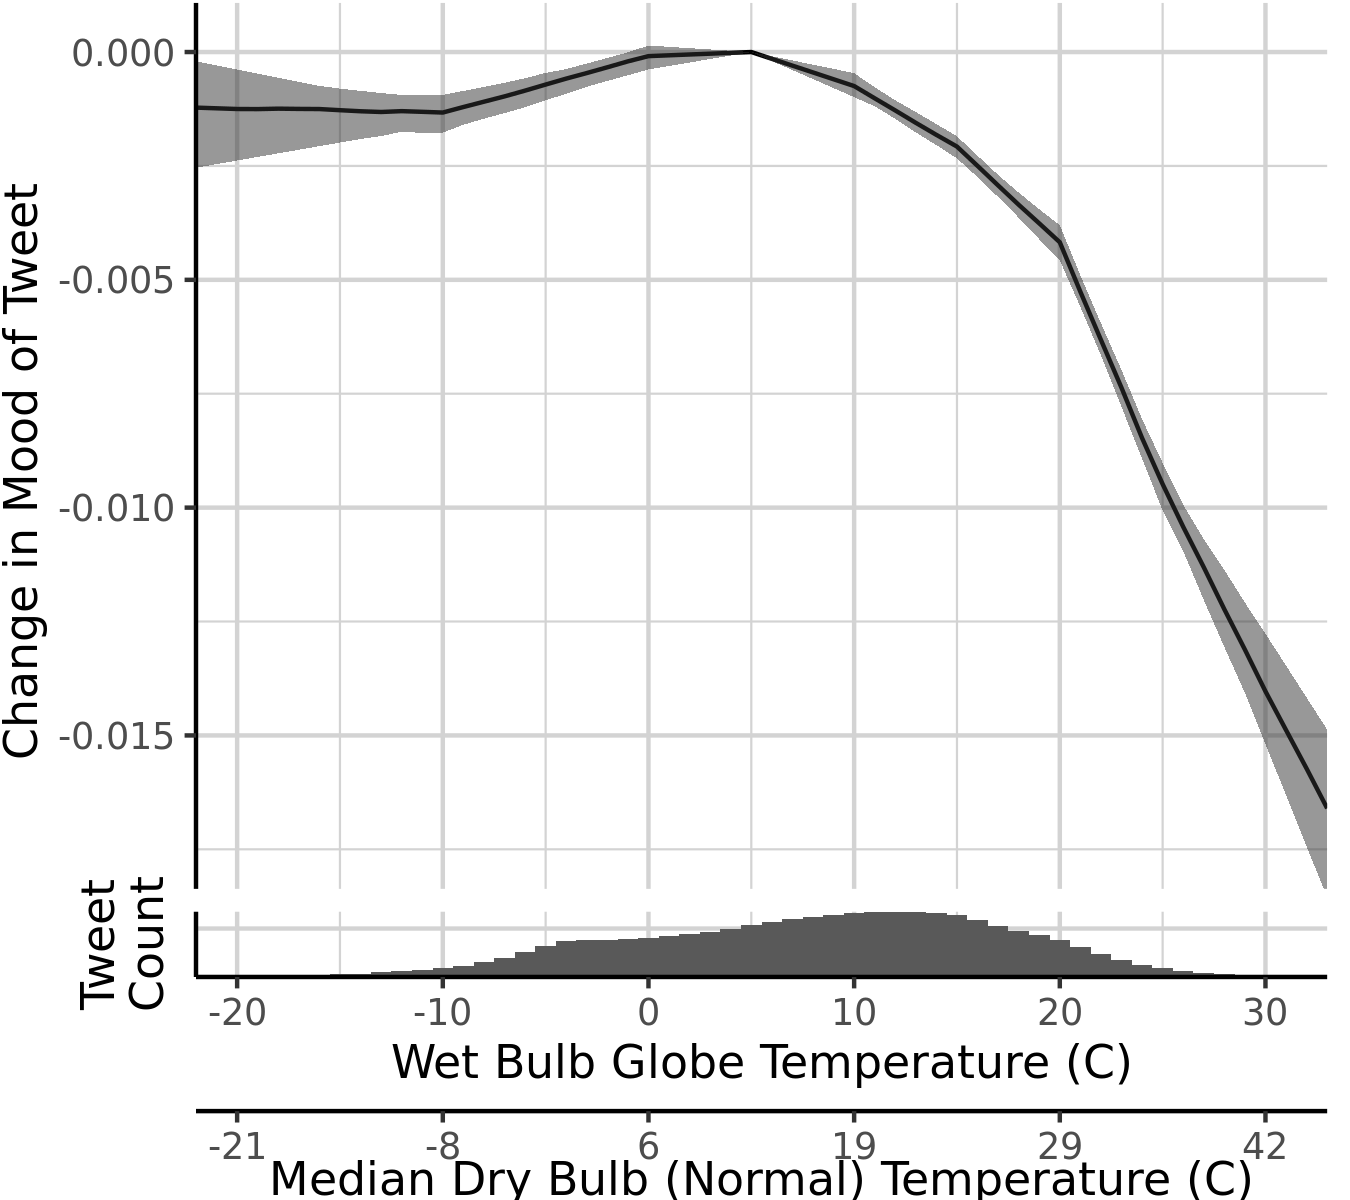
\includegraphics[width=0.5\linewidth]{../res/wbgt.png}
  \caption{Relationship between Wet Bulb Globe Temperature (WBGT) and sentiment in tweets.  As temperatures increase, sentiment declines.}
  \label{fig:wbgt}
\end{figure}

We then explored how the racial and income characteristics of neighborhoods moderate the relationship between WBGT and sentiment (See Fig \ref{fig:sub1}).  We found that neighborhood income strongly moderates the relationship between temperature and sentiment.  As temperatures increase to moderate heat of 20\textdegree C WBGT (29\textdegree C/84\textdegree F), sentiment decreases for most neighborhoods, but increases in neighborhoods in the 95th income percentile.  These rich do not see decreases in sentiment until temperatures are above 20\textdegree C WBGT (29\textdegree C/84\textdegree F), at which point sentiment decreases evenly across income ranges, still leaving a large gap in expressed sentiment from low to high-income neighborhoods.

We examined patterns of temperature and sentiment for neighborhoods that had a majority population of four broad racial categories - non-Hispanic black, non-Hispanic white, Hispanic of any race, and other, which includes Native American, multi-racial, and Asian-American and Pacific Islander.  While people in neighborhoods of all racial compositions were affected by heat, people in majority black neighborhoods were much more affected than others  (See Fig \ref{fig:sub2}).  Relative to an optimum temperature of 5\textdegree C WBGT (12\textdegree C/54\textdegree F), as temperatures increase to 30\textdegree C WBGT (42\textdegree C/108\textdegree F), the sentiment of tweets in majority black neighborhoods decreases four-times as much as people in other neighborhoods.  Additionally, at levels of moderate heat from 10\textdegree C WBGT (19\textdegree C/66\textdegree F) to 25\textdegree C WBGT (36\textdegree C/97\textdegree F), people in majority Hispanic neighborhoods have slightly lower sentiment than people in majority white or other neighborhoods, although this gap closes with high temperatures.

Finally, we modeled the combined effects of race and income in moderating the impacts of heat on mental health, and we found separate effects for these two variables (See Supplement).  In other words, neither race or income alone account for all the heterogeneity in vulnerability, and neighborhoods that are poor and black are more affected by than than neighborhoods that are just poor or just black.

\begin{figure}[H]
\centering
\begin{subfigure}{.5\textwidth}
  \centering
  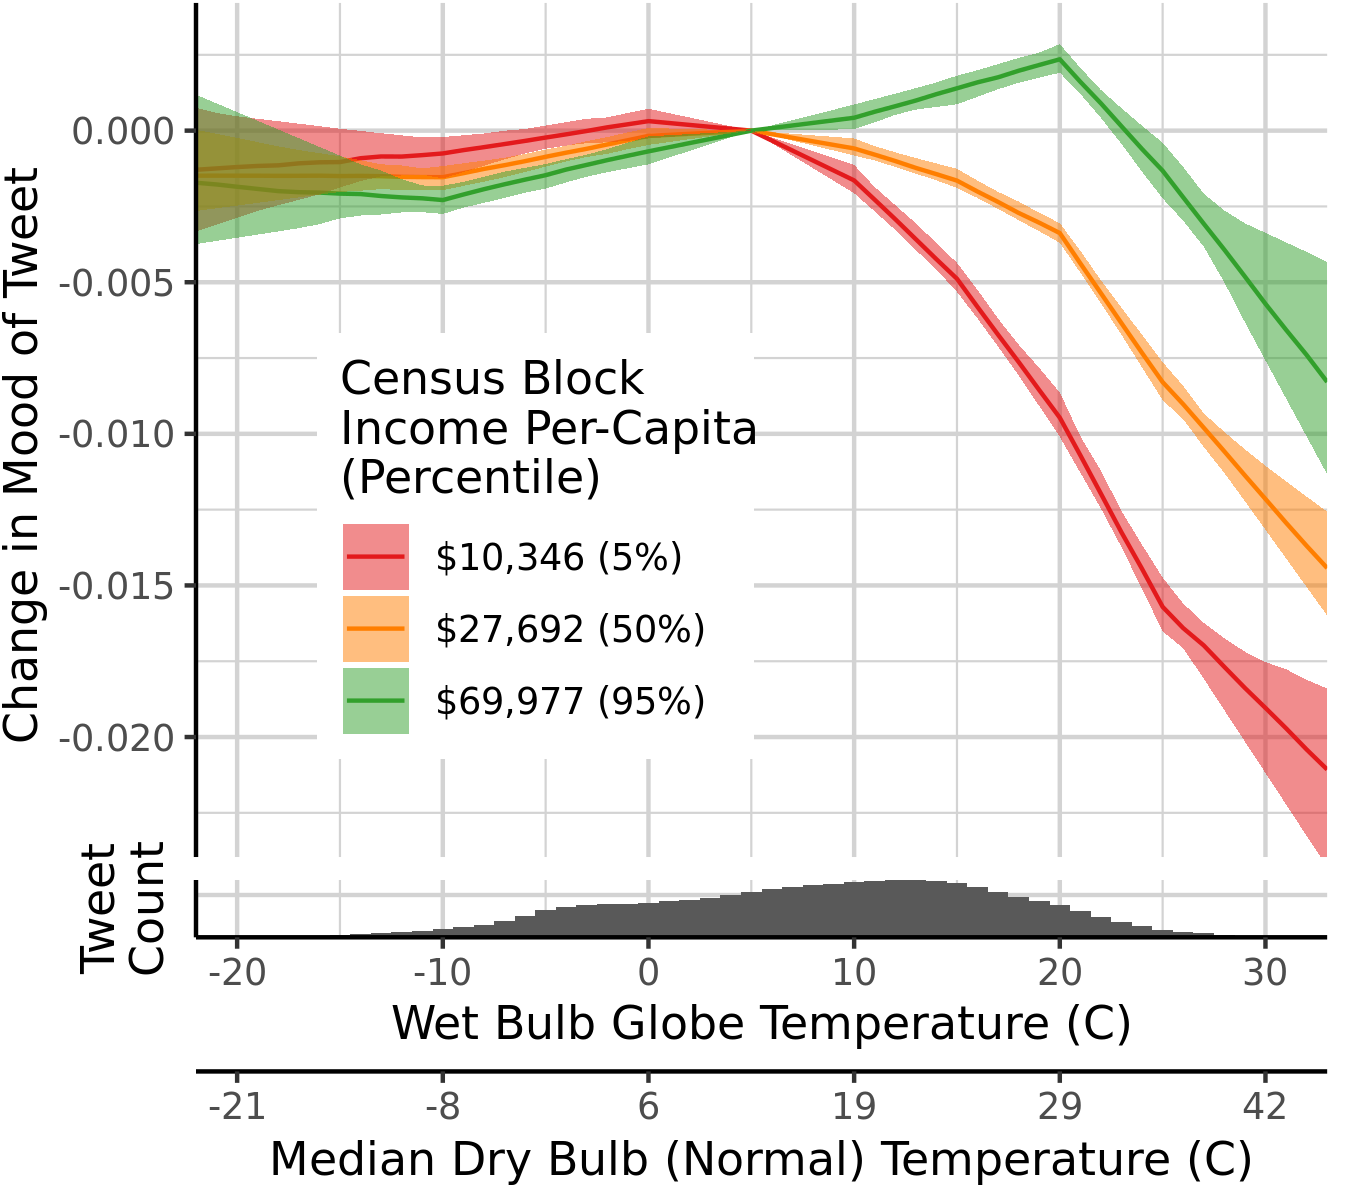
\includegraphics[width=\linewidth]{../res/wbgt-income.png}
  \caption{}
  \label{fig:sub1}
\end{subfigure}%
\begin{subfigure}{.5\textwidth}
  \centering
  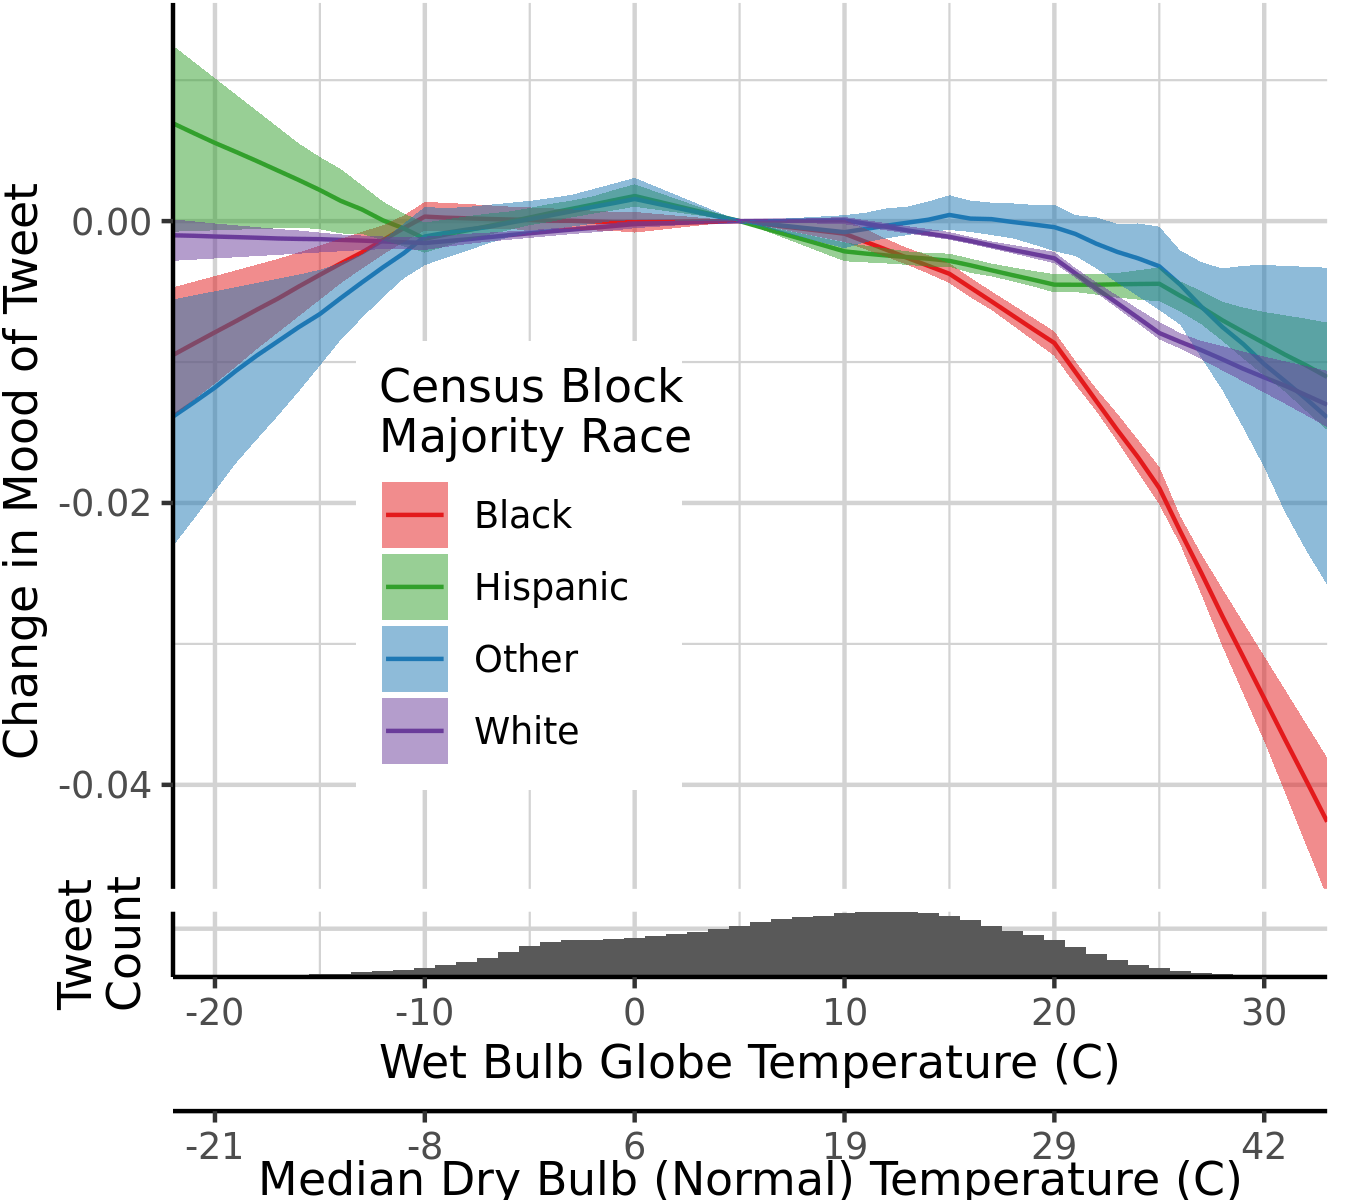
\includegraphics[width=\linewidth]{../res/wbgt-race_q.png}
  \caption{}
  \label{fig:sub2}
\end{subfigure}
\caption{Effect of changes in wet-bulb globe temperature on expressed sentiment relationship as moderated by neighborhood income (a) and race (b).}
\label{fig:test}
\end{figure}


\subsection{Comparison With Other Events}

Expressed sentiment is a widely used metric to assess mental health and well-being on social media.  While a variety of related metrics can be used to quantify sentiment, we chose to use the VADER metric that was specifically designed for microblogs like twitter \cite{hutto2014vader}.  To give context to this novel metric, we compare the impacts of heat waves, defined as a change from 5\textdegree C WBGT (12\textdegree C/54\textdegree F) to 25\textdegree C WBGT (36\textdegree C/97\textdegree F), to other events that have large impacts on sentiment (See Fig. \ref{fig:compare}).  Firstly, we examine the change in average sentiment from Saturday to Monday, the highest and lowest days for twitter sentiment as well as other mental health metrics, such as suicides.  We also examine the decrease in sentiment associated with the two most expensive hurricanes in the last decade in the United States.  For the hurricanes, we compared the mean sentiment of counties affected by Hurricanes Harvey and Sandy on the day of landfall to the mean sentiment a week before.  These hurricanes are associated with mental health effects including Post-Traumatic Stress Disorder (PTSD) \cite{Schwartz2017Aug, Schwartz2018May}, and similar disasters have been associated with subsequent increases in suicides \cite{Krug1998Feb}.

\begin{figure}[H]
  \centering
  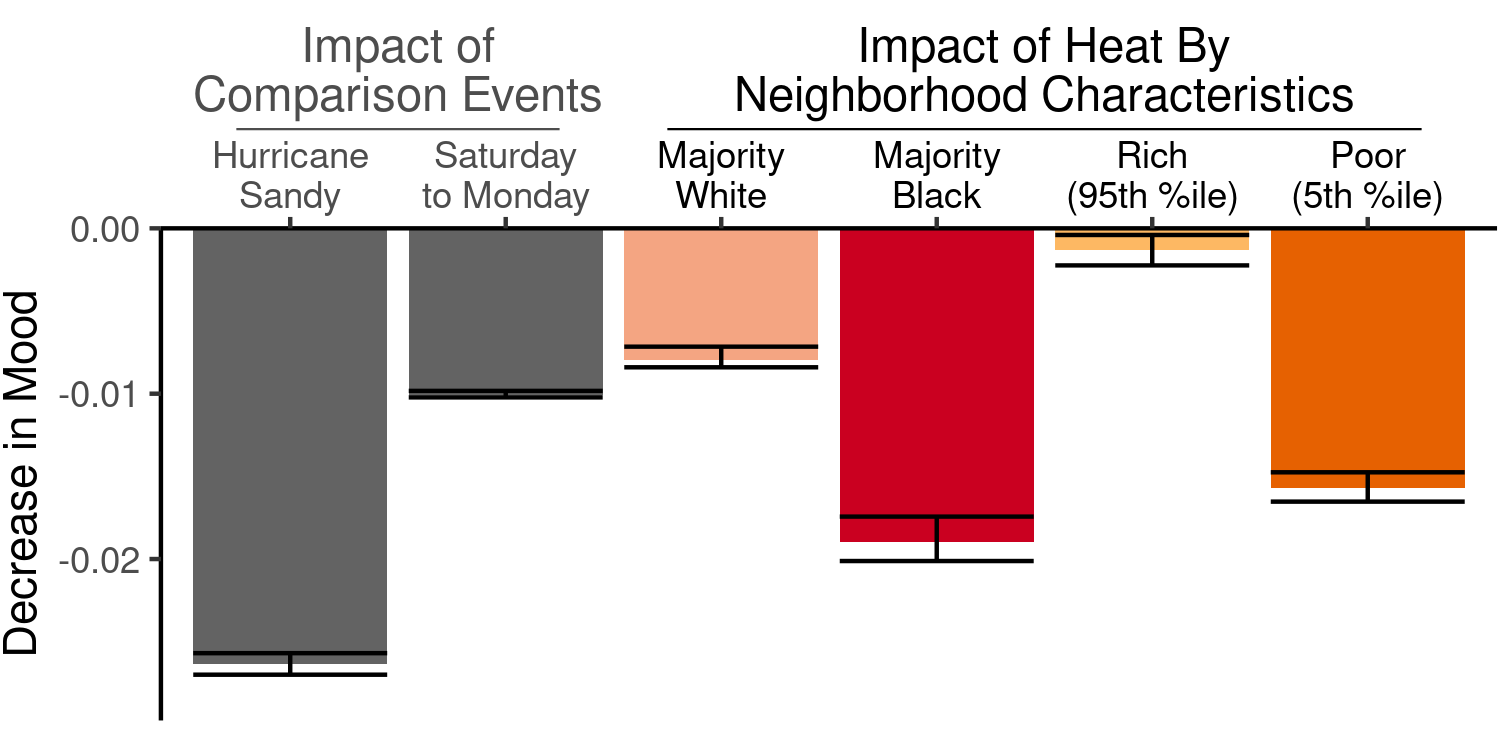
\includegraphics[width=\linewidth]{../res/comparison_plot.png}
  \caption{Decline in sentiment during a heat wave across several different neighborhoods, compared with other impacts on sentiment, such as major hurricanes, as well as the weekly variation in sentiment from the peak on Saturday to the low on Monday.}
  \label{fig:compare}
\end{figure}

We found that the impacts of heatwaves on sentiment in rich and majority white neighborhoods were less than the average weekly change in sentiment from Saturday to Monday, but the effects of heat waves on majority black or poor neighborhoods were much greater than the average weekly change in sentiment.  Additionally, the impacts of heat waves more vulnerable neighborhoods were close in degree to the impacts of both hurricanes.

{\color{red} What other disasters/comparison events should we look at?}

\subsection{Effects by Combined Statistical Area}

To further explore our findings, we examined inequalities in the impacts of higher temperatures on sentiment by Combined Statistical Areas (CSAs) and Metropolitan Statistical Areas (MSAs) with over 1 million people (hereafter: cities).  We examined the change in size of the gap in sentiment scores between both poor and rich neighborhoods, as well as black and non-black neighborhoods, as temperatures change from optimum temperatures of 5\textdegree C WBGT (12\textdegree C/54\textdegree F) to 30\textdegree C WBGT (42\textdegree C/108\textdegree F).

We found increasing inequalities in sentiment across income groups for 68.8\% of cities, with 35.6\% of these having a statistically significant effect (15 cities).  Cities with a significantly unequal effect were found in the south, Midwest, northeast, northwest, and southwest, although they were most common in the mid-Atlantic region.  Additionally, many cities in the southwest had an inverted effect, where higher temperatures actually narrowed the gap in sentiment between rich and poor neighborhoods, including Denver and Oklahoma City, which had a statistically significant inverted effect.

Because we found a much stronger effect for the effects of temperature on sentiment in majority black neighborhoods, we also examined increases in sentiment gaps between black and non-black neighborhoods in cities with a black population greater than 5\% of the total population.  We found increasing inequalities in sentiment for more black neighborhoods in 64.7\% of cities, with a significant effect in 21.2\% of those (7 cities).  Additionally, three sunbelt cities had a significant inverted effect.  The patterns of inequalities in the impacts of heat on sentiment by race were similar to inequalities by income: cities with large and significant inequalities were found the mid-Atlantic and Midwest, as well as central Florida.

\begin{figure}[H]
\centering
\begin{subfigure}{0.75\textwidth}
  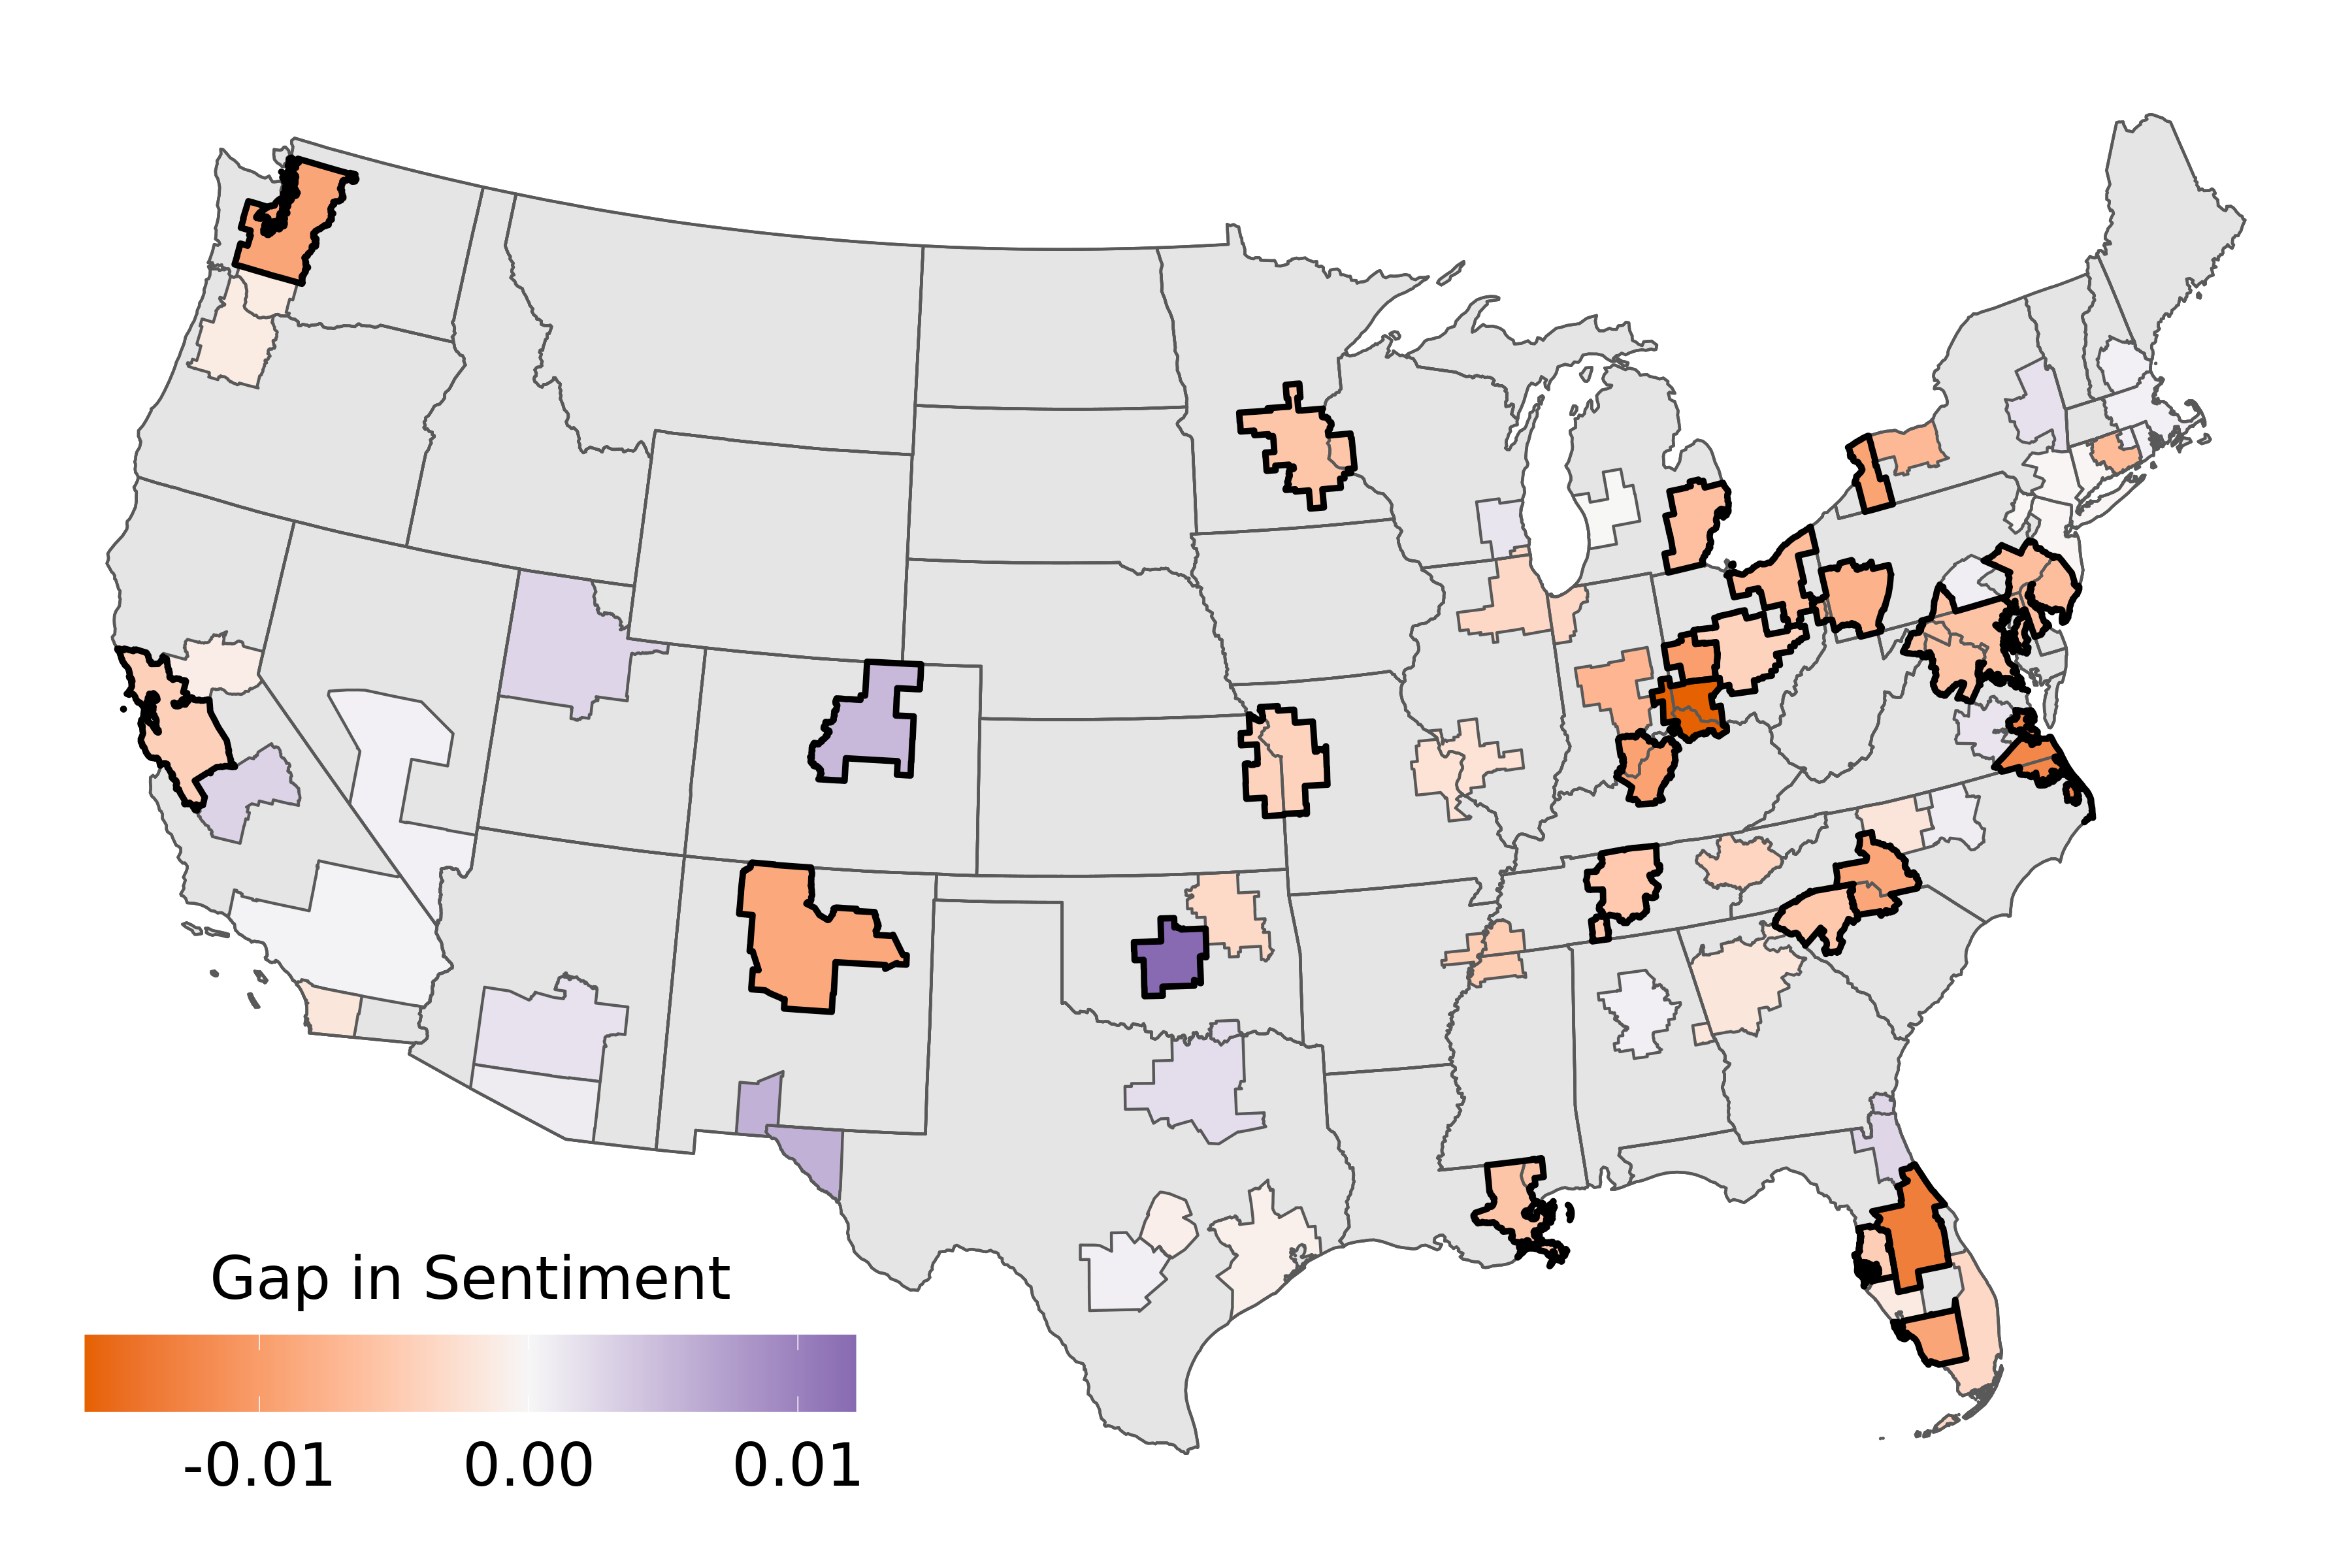
\includegraphics[width=\linewidth]{../res/map_wbgt_income.png}
  \caption{}
  \label{fig:map1}
\end{subfigure}
\begin{subfigure}{0.75\textwidth}
  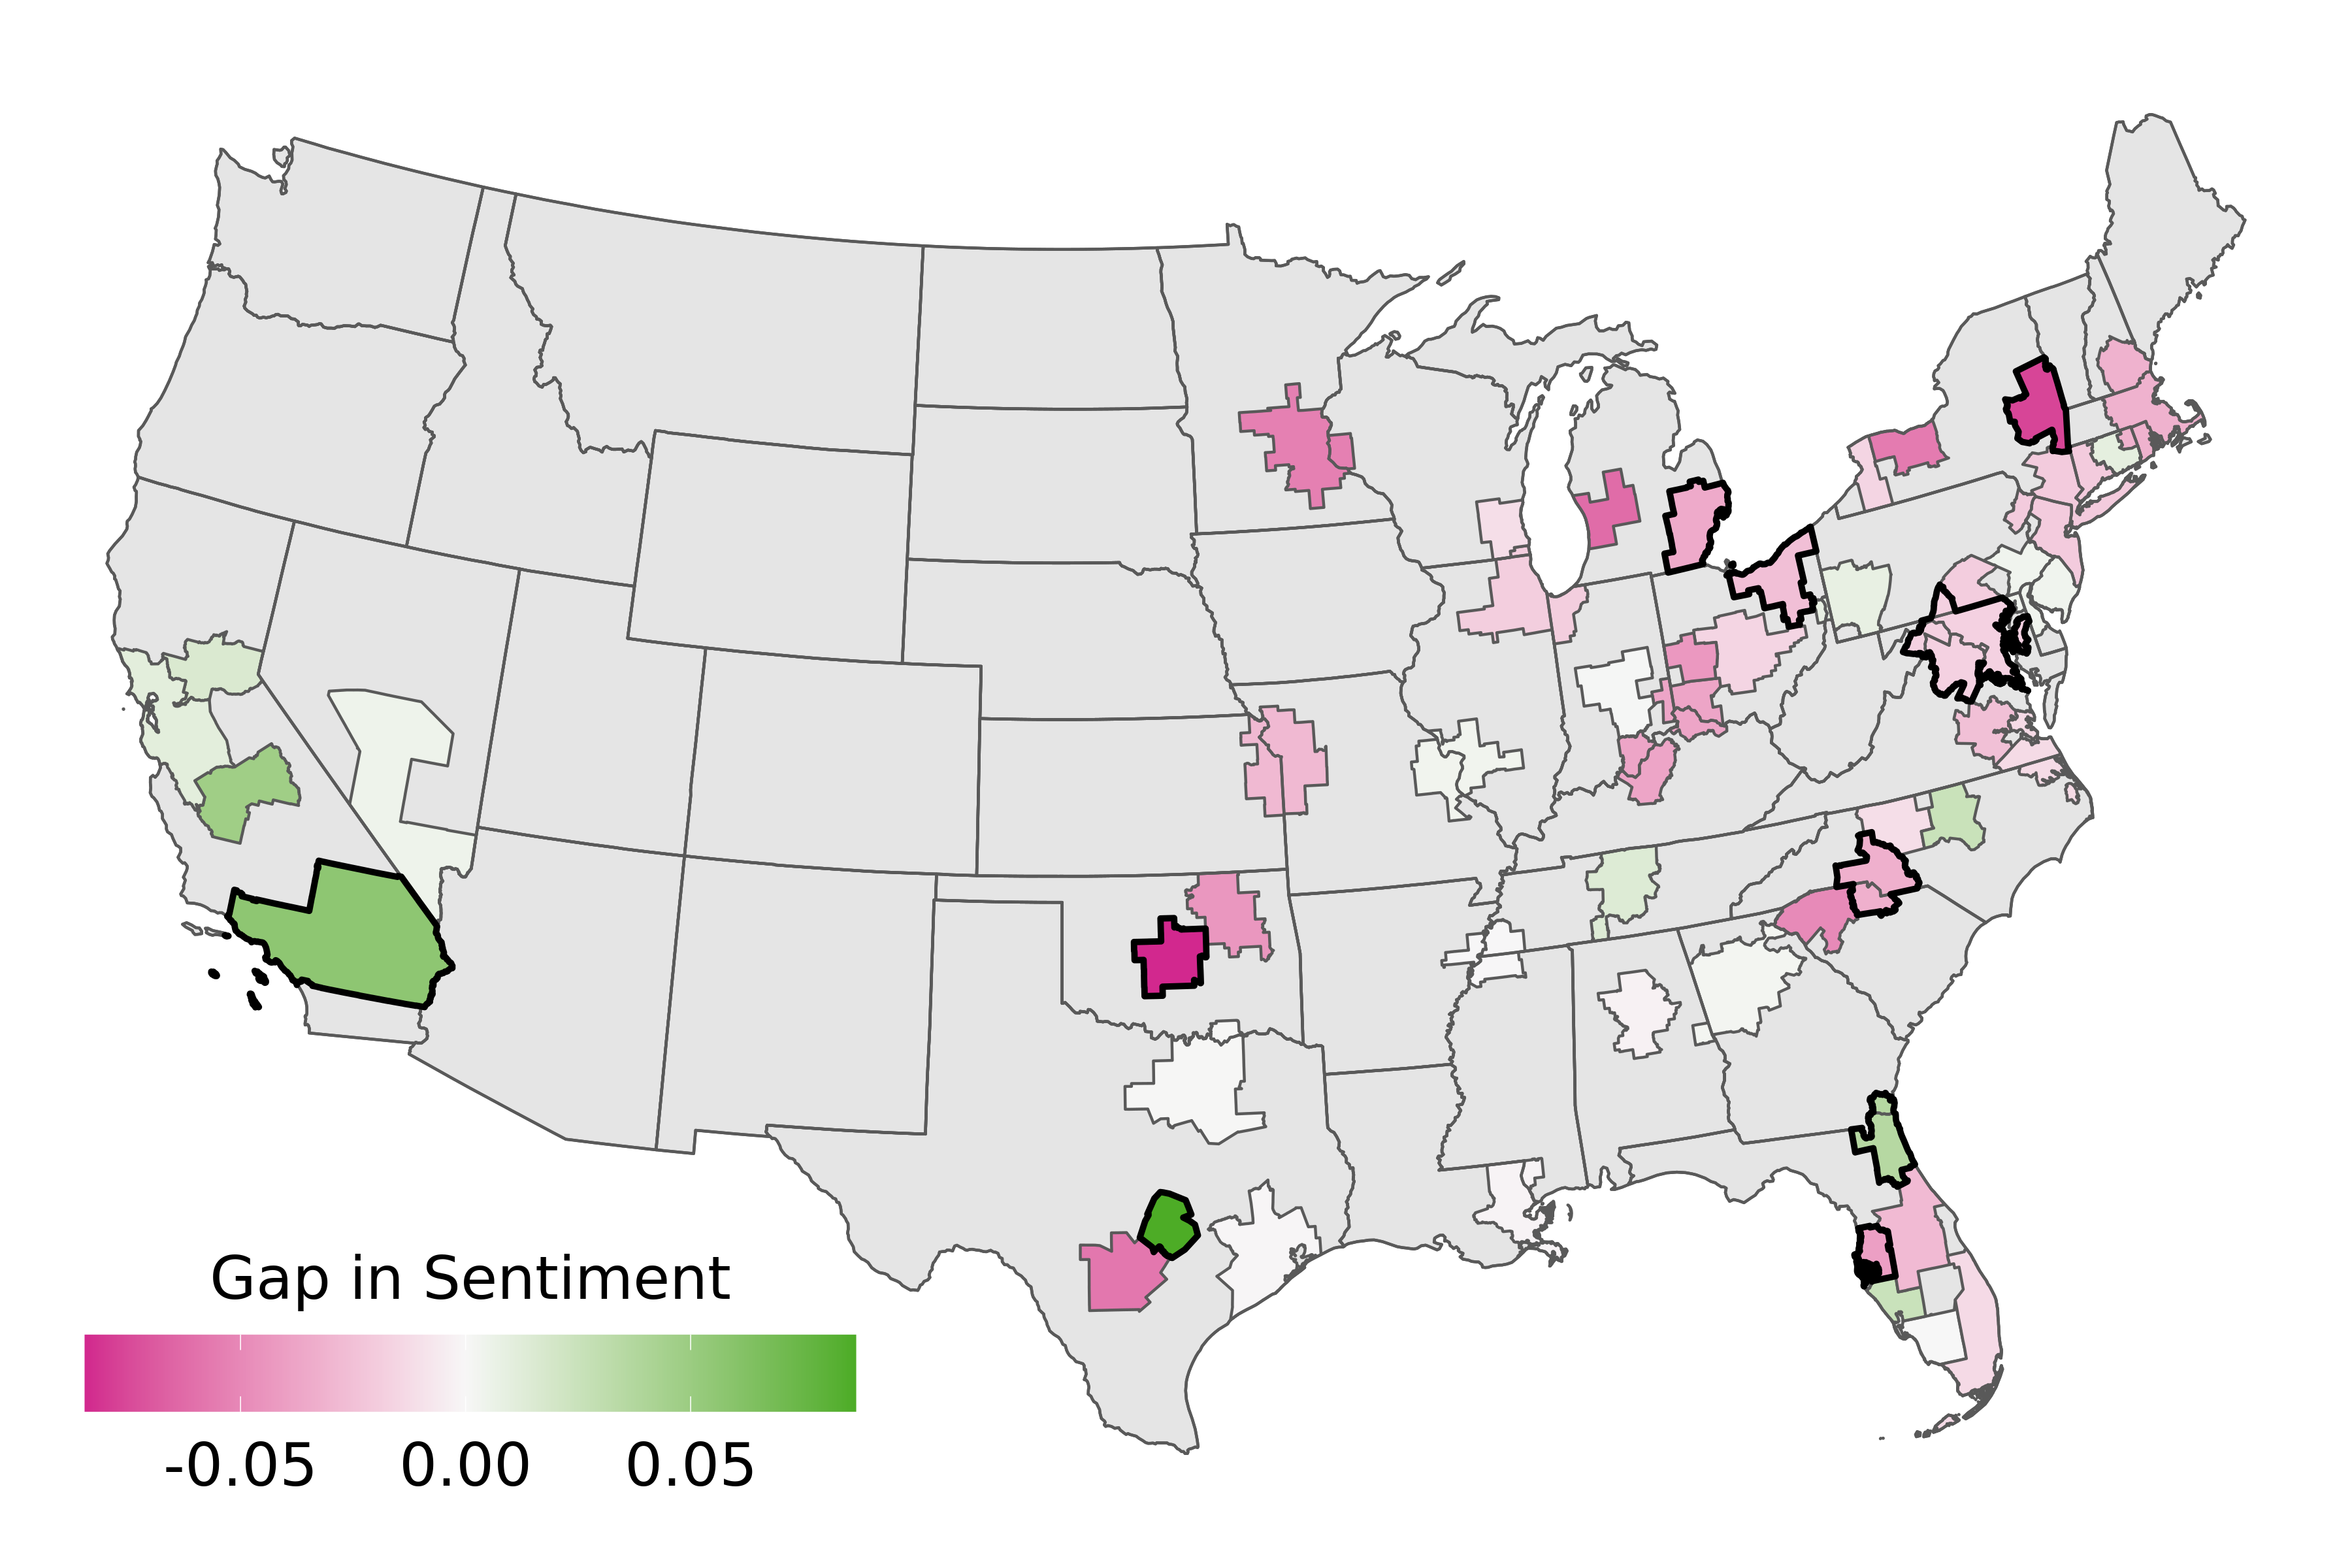
\includegraphics[width=\linewidth]{../res/map_wbgt_black.png}
  \caption{}
  \label{fig:map2}
\end{subfigure}
\caption{Inequalities in impacts of temperature on sentiment by CSAs and MSAs with over 1 million people.  The value shown is the predicted change in the size of the gap in VADER score as temperatures increase from 5WBGT to 30WBGT between the 5th and 95 percentile for income (a) and the 95th and 5th percentile for percent black (b).  CSAs with a statistically significant effect ($p < 0.05$) are outlined in black.  For racial inequalities (b), only MSAs and CSAs where black people make up $> 5\%$ of the population are included.}
\label{fig:test}
\end{figure}

\section{Discussion}
% Benefits of twitter data/overview of findings
We found that twitter data offers significant advantages for observing environmental effects on human well-being due to its very fine spatio-temporal resolution.  We were able to pair each tweet with the local temperature at the time of the tweet, and found a clear association between heat and worsened sentiment.   Moreover, we were able to show clear heterogeneities in vulnerability by neighborhood characteristics, overturning previous findings that found no heterogeneities at the county level \cite{Burke2018Aug, Mullins2019Dec}.

% Sentiment is a fuzzy indicator but we have BIG DATA
However, one limitation of data from twitter is that a tweet is not a precise measurement of a discrete mental health outcome and only provides a rough indicator a user's mental state based on the vocabulary in the tweet.  Moreover, while sentiment analysis algorithms have gotten increasingly sophisticated at estimating the mood in a body of text, a user's expressed sentiment in a tweet is highly variable and is mostly affected by factors like current events and the user's personal life, with local weather conditions having only a small impact.  We overcome this limitation by using an extremely large data set of nearly 250 million tweets, allowing us to control for a wide variety of spatial and temporal effects to estimate population-level changes in sentiment in relation to the weather.

% Compare weekly changes in sentiment to weekly changes in suicides
We found that the change from optimum temperature of 5\textdegree C WBGT (12\textdegree C/54\textdegree F) to a heatwave of 25\textdegree C WBGT (36\textdegree C/97\textdegree F) is associated with an overall decrease in the VADER sentiment score of 0.01.  This is similar to the degree of change in sentiment over the course of a week from a Monday nadir (0.1268) to a Saturday peak (0.1372), a weekly change associated with a increase in suicides of 23\% over the course of the study period \cite{CDC2021}.  Thus, while research on linkages between sentiment and other mental health outcomes like suicides and hospitalizations is still nascent, there are clear similarities in patters of sentiment and suicides at some time scales.  Moreover, both suicides and sentiment are affected by higher temperatures \cite{baylis_weather_2018, Burke2018Aug}.  Thus, while twitter sentiment is the only mental health indicator available at fine enough spatial and temporal scales to examine neighborhood effects, these changes in sentiment are representative of real human suffering, and are also very likely indicative of medical outcomes like suicides and hospitalizations, although this analysis cannot speak to those outcomes specifically.

% Discuss the NOVELTY: quote Burke and Mullins, refute their interpretations, people have said XX, but we have shown ~XX.
% Variations in vulnerability also indicates ADAPTATION
Previous work conducted with county-scale data found no heterogeneities in mental health vulnerability by income.  Such analyses have led to conclusions that (1) the mental health effects of climate change will be uniform, least in developed countries, and (2) that adaptation with technologies like air-conditioning will not be enough.  For example, Mullins et al. conclude that ``high-temperature events will harm mental health everywhere" and that ``individuals have not been able to successfully reduce the negative effects of higher temperatures on mental health" \cite{Mullins2019Dec}.  Contrary to these analyses, we found large heterogeneities in vulnerability by neighborhood race and income.  This suggests that the mental health effects of climate change will not be uniform and, like other impact, will fall disproportionately on the poor and vulnerable.  More positively, it does suggest that adaptation is possible, and, for communities with infrastructure and working conditions similar those of high-income Americans, the effects of high temperatures on mental health can be largely mitigated.

% Comment on interpretation of results
We examined our results relative to an optimal baseline temperature of 5\textdegree C WBGT (12\textdegree C/54\textdegree F), as this was the temperature at which the highest sentiment scores were observed in the aggregated analysis (See Fig. \ref{fig:wbgt}).  However, after examining heterogeneities by neighborhood race and income, we find different optima for different racial groups and income levels.  For example, the optimum temperature for poor neighborhoods is 0\textdegree C WBGT (6\textdegree C/43\textdegree F) while the optimum temperature for rich neighborhoods is 20\textdegree C WBGT (29\textdegree C/84\textdegree F).  These different varying optima show that even mild heat can affect human well-being, and the only reason that sentiment peaks as high as 20\textdegree C WBGT (29\textdegree C/84\textdegree F) in rich neighborhoods is because the rich are more likely to have air conditioning in their homes, transportation, and work spaces, as well as much greater choice in when they are outside and in the activities they perform outside.

% Comment on Race, why no effect on hispanics?
We found that majority black neighborhoods are much more affected by heat than neighborhoods with a majority of any other race.  This is surprising, given that Hispanics can be marginalized in both income and housing.  This finding may be because the racial category of Hispanic is more broad and encompasses many more groups with more diverse histories and income levels than black Americans, or may also be due to that fact that more marginalized and heat-vulnerable Hispanic people were more likely to tweet in Spanish, which we excluded from our analysis.  Additionally, there are many other marginalized groups in America, particularly indigenous people, that we did not have sufficient data to examine with respect to heat and mental health.  

% Interpret Spatial Analysis
In our spatial analysis, we found that heat affects sentiment in cities across the US, suggesting that higher baselines temperatures do not reduce vulnerability.   Additionally, most cities exhibited both racial and income inequalities in the vulnerability of mental health to heat, although the south-west had the weakest inequalities and an occasional inverted effect.  While this could suggest that heat inequality is related humidity, this is unlikely because we used Wet Bulb Globe Temperature, which accounts for how differences in humidity and wind speed affect the human body's ability to cool itself through perspiration.  Thus, this regional differences in vulnerability are likely more due to cultural or infrastructural differences than to different baseline environmental conditions.

% Interpret Time Series Analysis
Recent research has suggested that the impacts of heat on sleep quality may play a large role in the observed mental health effects of heat \cite{Obradovich2017May, Mullins2019Dec}, and our temporal analysis was able to examine this hypothesis.  While our estimates were more uncertain at night due to a lower volume of tweets, we found much stronger effects of heat on expressed sentiment in the early morning, adding weight to the sleep quality pathway linking heat and mental health that other authors have found.  This suggests that efforts to improve mental health during heat waves may have the largest impact by focusing on providing electricity and air conditioning at night.

% Caveats
While these findings are robust to different model specifications and sentiment metrics, there are some caveats.  For one, we were only able to locate the tweets within the census block where the tweet was sent - we did not to infer where the person sending the tweets typically lived or where they had been.  Many low-income and black people commute during the day to work in the service sector in higher-income areas, so these results may in fact under-estimate the impacts of higher temperatures on mental health for poor and minority individuals.  Moreover, the income level of a census block may be only weakly correlated with the wealth of the people who are typically found that census block.  For example, some public spaces are estimated to have very low income levels even though people from a variety of income levels may occupy those spaces throughout the day.  Additionally, neighborhoods of young college students are also typically estimated to have low income levels, even through college students are wealthier than the average American.  Again, these issues mean we are likely under-estimating the true effect of heat on mental health.  A final issue with using twitter data is that, while twitter is used by more than one in five Americans, twitter users may not be representative of the general population, as they are typically younger, wealthier, and more educated \cite{Pew2020Sep}.  Nevertheless, we found a large volume of tweets across all neighborhood types.

% NCC doesnt have a "conclusion" section, but this is intended as an overall summary paragraph
While climate change will have widespread and severe impacts on human well-being, it cannot be overemphasized just how highly unevenly these impacts will be distributed.  People with more money, access to aid and infrastructure, and who belong to ethnic groups in power are less affected by climate shocks and natural disasters and more able to adapt \cite{bullard2012wrong}.  While the physical health impacts of these shocks are more visible and easy to measure, the mental health impacts of climate change are also causing severe human suffering and there is no reason to believe they are not also highly unevenly distributed.  Thus, there are strong theoretical priors behind the hypothesis that low-income and marginalized people are more vulnerable to the mental health impacts of higher temperatures, even though previous work at coarse spatial scales has not found such an effect.  By using fine-scale twitter data, we showed that there are indeed stark difference in the mental health impacts of heat among neighborhoods in the United States.  These findings have significant implications for urban planning, climate and environmental justice, and mental health.

\section{Methods}
\subsection{Tweets \& Sentiment}
We used data from 243 million geo-located English-language tweets from the lower 48 states from the years 2009 to 2019.  The Twitter data consists of publicly posted messages, or Tweets, that are short status messages users post to the platform.  We only considered users’ original content, thus did not include retweets in our analysis.  Additionally, we excluded all tweets that contained weather-related terms, to ensure that the sentiment expressed in the tweets was reflective of a user's mental state, and not a commentary on the weather.

We assessed the sentiment expressed in the tweets using the VADER (Valence Aware Dictionary for sEntiment Reasoning) sentiment corpus \cite{gilbert_vader_2014}. VADER is a lexicon and rule-based sentiment analysis tool that is specifically attuned to sentiments expressed in social media because of several features, as:

\begin{itemize}
  \item Incorporating lexical features common to informal media, such as slang (``sux"), and acronyms (``lol").
  \item Negations (``\textit{not} good", ``\textit{wasn't} bad")
  \item Punctuation (``Good!!!")
  \item Word shape, such as capitalization (``The move was AMAZING")
  \item Emoticons and emojis (``:-)", ``\emojismile")
  \item Degree modifiers (``very excellent" or ``kind of crappy")
\end{itemize} 

The VADER method yields a value for the mood of a tweet, with a score of 0 for neurtral tweets, a score $> 0$ for positive-mood tweets and a score $< 0$ for negative-mood tweets.  In addition to the VADER method used in the body of this paper, we also conduct our analysis using the Hedonometer and AFINN sentiment analysis methods, with similar results (See Supplement).

\subsection{Weather}
We used data on local weather conditions from the North American Land Data Assimilation System (NLDAS), a gridded product developed by several collaborative institutions, including NOAA, NASA, Princeton University, and the University of Washington.  This dataset is available at an hourly temporal resolution, and at 1/8th decimal degree spatial resolution, and integrates a large quantity of observation-based and modeled data  \cite{xia_continental-scale_2012}.  For the exact hour and location of each tweet, we extracted temperature, specific humidity, air pressure, total precipitation, shortwave radiation, and wind speed.  

Because metrics of apparent temperature that take into account humidity and other factors can better account for the impacts of heat stress on human health and wellbeing, we calculate the Wet Bulb Globe Temperature (WBGT) at the time and location of each tweet.  WBGT is the temperature that a wet globe thermometer would read in direct sunlight, and gives a reading lower than a dry bulb temperature would show due to evaporative cooling, and can be estimated given normal temperature, relative humidity, solar radiation, and wind speed.  Because evaporative cooling is how humans cool themselves through perspiration, this temperature better indicates the heat stress that people are experiencing.  Metrics like WBGT that account for the effects of humidity and other factors on heat stress have been associated with diminished economic output \cite{rao2020projections}, increased crime \cite{hu2017impact}, increased mortality \cite{chien2016spatiotemporal, armstrong2019role}, and worsened mental health outcomes \cite{vida2012relationship, ding2016importance}.

Using temperature, specific humidity, and pressure, we derived relative humidity using methods described by  \cite{bolton_computation_1980}.  We then calculated the WBGT using the formula described by \cite{heo2019comparison}.

\subsection{Socio-Econoimc Data}
We used data from the American Community Survey (ACS) administered by the US Census to estimate income levels and the racial composition of neighborhoods where tweets were located.  Data was at the level of the census block group, the smallest unit for which the census releases public data.

ACS data is released to cover five-year periods.  We therefore matched each tweet with census block group data from the year at the middle year of each survey's five-year range.  For example, tweets from 2014 were matched to data from the 2012-2016 ACS.  Because the most recent available ACS was from 2014-2018, all tweets from year years greater than 2016 were matched to this dataset.  Data was downloaded from the IPUMS NHGIS service provided by the University of Minnesota.

Mean annual income per capita is provided by the ACS, and we standardized this variable so that the values for each year were in 2019 dollars.  For racial categories, we combined the various categories provided by the ACS into four racial groups: non-Hispanic white, non-Hispanic black, Hispanic of any race, and an "other" category for non-Hispanic people who were neither black nor white, such as Asian, Native American, or mixed-race people.

\subsection{Modeling}
We assessed how expressed sentiment is affected by wet bulb globe temperature using segmented regressions, controlling for precipitation, and shortwave solar radiation (sunshine), as well as the following spatio-temporal fixed effects: the day of the week, the time of day, the day of the year, the year, the month, and the county.  

Our initial model (for Fig. \ref{fig:wbgt} takes the following form:

\begin{equation}
    y = \beta_0 + f_t(t) + \beta_p p + \beta_s s + \Phi + \epsilon
\end{equation}

Where $y$ is the sentiment of a tweet, $t$ is the wet bulb globe temperature at the hour of the tweet, $p$ is a binary variable indicating whether it rained at the hour of the tweet, $s$ is the income shortwave radiation, or sunshine, in $W/m^2$, at the hour of the tweet, $\Phi$ is the spatio-temporal fixed effects, $\epsilon$ is the normally-distributed errors, and $f_t$ represented the segmented regression for $t$, with knots at -10\textdegree, 0\textdegree, 5\textdegree, 10\textdegree, 15\textdegree, 20\textdegree, and 25\textdegree C WBGT.  We estimate the 95\% confidence interval of our models using 80-fold bootstrapping.  

To examine how income and racial groups moderate the effect of heat on sentiment, we extend our model to the following form:

\begin{equation}
    y = \beta_0 + f_t(t) + f_{mt}(m t) + \beta_p p + \beta_{mp} m p + \beta_s s + \beta_{ms} m s + \Phi + \epsilon
\end{equation}

Where $m$ is either the log-transformed average income in the census block where the tweet originated, or a dummy variable for the four racial categories.  We specify alternative models where income is a dummy variable in three bins, and were race is a continuous variable for the percent of a census block population that is what.  These alternative specifications yield similar results.  We also examine the effects of rainfall and sunshine on sentiment by income and race.  These alternative specifications and analysis of rainfall and sunshine effects are available in the Supplement.

For our analyses by CSA, we subset the data in the model and run the model with the same fixed effects, although we fit a linear effect for $f_t()$.


\section{Acknowledgements}
%Official SESYNC wording
This work was supported by the National Socio-Environmental Synthesis Center (SESYNC) under funding received from the National Science Foundation DBI-1639145.  Additionally, cloud resources for this project were provided for the Microsoft Azure cloud by Microsoft's AI for Earth program, grant number .

This data came from Twitter via the University of Vermont’s (UVM) agreement with Twitter to access its streaming API - colloquially referred to as the Decahose.  The UVM special agreement with Twitter allows for access to this data for research and analysis purposes and we have complied with all the terms of service for Twitter and UVM. 
\printbibliography

\section{Author Contributions}
Author contributions: M.W.C. and P.B. designed research and modeling strategy; A.S. provided data; M.W.C and Z.L. prepared data; M.W.C. and J.O.G analyzed data; and M.W.C., J.O.G., J.L., and P.A.W. wrote the paper.

This project was co-lead by M.W.C. and J.O.G.

\end{document}
